\documentclass{article}

\usepackage{geometry}
\geometry{a4paper}
\setlength{\parindent}{10mm}
\setlength{\parskip}{0.9em}
\def\baselinestretch{1.5}

\usepackage[spanish,mexico]{babel}
\renewcommand {\spanishtablename}{Cuadro}
\usepackage[spanish,onelanguage,ruled]{algorithm2e}
\usepackage[utf8]{inputenc}
\usepackage{graphicx}
\usepackage{caption} 
\usepackage{amsmath, amsthm, amsfonts}
\usepackage{enumerate} 
\usepackage{fancyhdr}
\usepackage{anysize} 
\usepackage[usenames]{color}
\usepackage{booktabs}
\usepackage{etoolbox}
 \usepackage{fancyvrb}
 \usepackage{color,soul}
 \usepackage[dvipsnames]{xcolor}
 \usepackage{graphicx}
\usepackage{subcaption}
\usepackage{listings}
\usepackage{amssymb}
\usepackage{multirow}


\usepackage{verbatim}
% redefine \VerbatimInput
\RecustomVerbatimCommand{\VerbatimInput}{VerbatimInput}%
 {fontsize=\footnotesize,
  %
  frame=lines,  % top and bottom rule only
  framesep=1em, % separation between frame and text
  rulecolor=\color{Gray},
  %
  label=\fbox{\color{Black}test.txt},
  labelposition=topline,
  %
  %commandchars=\ \mid \(\), % escape character and argument delimiters for
                  % commands within the verbatim
  %commentchar=*        % comment character
 }


\pagestyle{fancy}

\chead{}
\lhead{} 
\rhead{}
\lfoot{\it }
\cfoot{}
\rfoot{\thepage}

\title{
\centering
Modelos Probabilistas Aplicados \\
Johanna Bolaños Zúñiga \\
Matricula: 1883900\\
Tarea 8
}

\date{}

\begin{document}
\maketitle

\section{Discusión sobre material proporcionado en clase}
El teorema de Bayes permite que el proveedor de atención médica convierta los resultados de una prueba en la probabilidad de tener una enfermedad. Este teorema se utiliza para calcular la probabilidad condicional de un suceso, teniendo información de antemano de dicho suceso, en otras palabras, sirve para determinar la probabilidad de una de las causas, puesto que ya se observó el efecto o suceso, y se calcula de la manera siguiente:
\begin{equation}
P(A_{n} \mid B)= \frac{P[B \mid A_{n}]*P[A_{n}]}{\sum_{i=1}^{n}P[B \mid A_{i}]*P[A_{i}]},
\label{bayes}
\end{equation}
\noindent donde $B$ es el suceso sobre el que tenemos información previa, $A_{n}$ son los distintos sucesos condicionados y $A_{i}$ es la causa $i$, donde $i$ = $1, 2, 3, \dots , n$. Aplicando la la ley de la multiplicación a la ecuación \ref{bayes} se obtiene la siguiente expresión (ecuacion \ref{bayes1}):
\begin{equation}
P(A \mid B)= \frac{P[B \mid A]*P[A]}{P[B]},
\label{bayes1}
\end{equation}
\noindent donde en la parte del numerador se tiene la probabilidad condicionada, y en la parte del denominador la probabilidad total. 

De acuerdo a la enfermedad del Covid\textendash 19, hay diversos estudios donde se utiliza el teorema de Bayes para analizar los casos que se tienen al realizar la prueba y de los factores que influyen para su cálculo. Los casos que se pueden presentar son:

\begin{itemize}
    \item Verdaderamente positivos: si una persona con Covid\textendash 19 da positivo a este.
    \item Verdaderamente negativos: cuando una persona sin Covid\textendash 19 da negativo en las pruebas.
    \item Falsos positivos: cuando una persona sin Covid\textendash 19 da positivo a este.
    \item Falsos negativos: si una persona con Covid\textendash 19 da negativo en la prueba.
\end{itemize}

Para interpretar con una mejor precisión el resultado de la prueba, es necesario conocer su valor predictivo positivo (VPP)\footnote{El valor predictivo positivo (VPP) permite identificar el porcentaje de personas que tienen la enfermedad cuando la prueba ha dado positiva.} y negativo (VPN)\footnote{El valor predictivo negativo (VPN) de una prueba es la ``capacidad de descartar una enfermedad" dado un resultado negativo de la prueba.}, los cuales dependen de la sensibilidad y especificidad y la prevalencia o la probabilidad previa a la prueba (probabilidad a priori). Se conoce como sensibilidad de cualquier prueba biomédica a la probabilidad de que una persona dé positivo dado que tiene la enfermedad y, la especificidad a la probabilidad de que una persona dé negativo dado que no tiene la enfermedad. En el trabajo de Schnipper \cite{link1}, de manera interactiva muestran como calcular los VPP y VPN.

Por ejemplo, en la investigación de Lewis \cite{link2}, se utiliza el teorema de Bayes para demostrar cómo la calidad de una prueba de Covid\textendash 19 depende de la magnitud del brote (tasa base), en este estudio, reescriben la ecuación \ref{bayes1} usando las probabilidades relevantes para las pruebas de Covid\textendash 19 dando como resultado la ecuación \ref{link2},
\begin{equation}
P(Cov \mid Pos)= \frac{P[Pos \mid Cov]*P[Cov]}{P[Pos \mid Cov]*P[Cov] + P[Pos \mid NoCov]*P[NoCov]},
\label{link2}
\end{equation}
\noindent donde $P(Cov \mid Pos)$ es la probabilidad de que una persona tenga Covid\textendash 19 dado que ha dado positivo en la prueba, $P(Pos \mid Cov)$ es la sensibilidad de la prueba, $P(Cov)$ es la tasa base o la prevalencia (número de casos de Covid\textendash19 / número total de la población a analizar), $P(NoCov)$ el porcentaje de personas que no tienen la enfermedad, ($1-P(Cov)$) y $P(Pos \mid NoCov)$ es la probabilidad de los falsos positivos.

De acuerdo a la ecuación \ref{link2}, considero que es correcto determinar que, incluso cuando se utiliza una prueba muy sensible, cuanto menor sea la tasa base de la enfermedad, más probabilidad se tiene de obtener falsos positivos. Asimismo, entre mayor sea la tasa base, más probabilidad hay de obtener falsos negativos a medida que se aumenten las pruebas.

Por otro lado, en el trabajo realizado por Ranjan \cite{link3}, propone un modelo donde calculan el valor predictivo positivo VPP y la prevalencia o tasa base está determinada por la ecuación \ref{link3},
\begin{equation}
P= 1-(1-p)^x,
\label{link3}
\end{equation}
\noindent donde $P$ es la probabilidad de que al menos $1$ persona de las $x$ cantidad de muestras tenga Covid\textendash 19 y $p$ es la probabilidad de que $1$ persona tenga la enfermedad. En este trabajo, el hecho de que la prevalencia sea igual al número de casos de Covid\textendash19 dividido el número total de la población a analizar, demuestra que el cálculo del VPP, no es un indicador de gran ayuda para determinar el porcentaje de personas realmente están infectadas, aún sí se considera que las personas a evaluar viven en un área donde es más probable que contraiga el virus (zona roja), por lo tanto, la metodología propuesta en cuanto a determinar los verdaderos positivos con base en el número de muestras realizadas, no parece erróneo. Sin embargo, considero que el estudio realizado carece de claridad respecto a los resultados obtenidos.

En la investigación de Good \cite{link4}, aplican un análisis bayesiano (cálculo del VPP y VPN) para ilustrar la interpretación de las pruebas negativas de Covid\textendash 19 considerando que la prevalencia es la probabilidad previa a la prueba, es decir, una probabilidad con base en la sospecha clínica de padecer la enfermedad. Proponen dos escenarios (alta y baja probabilidad previa a la prueba de infección por Covid\textendash 19) clínicos. Para ambos escenarios, asumen una especificidad del $99,9\%$ y varían la sensibilidad del $70\%$ al $90\%$. Considero que los resultados obtenidos van acorde a la metodología planteada, puesto que se realizó de manera correcta la interpretación de los VPN y VPP.

Finalmente, en la investigación de Chan \cite{link5}, se realiza el estudio basado en las razones de verosimilitud negativa (LR$-$, por sus siglas en inglés de, \textit{negative likelihood ratio}) y de odds (razón de probabilidades), los cuales son posibles de calcular utilizando el teorema de Bayes y, la prevalencia o probabilidad previa de la prueba es una probabilidad a priori, es decir, con base en la experiencia del médico y la información que posee acerca de la enfermedad en particular del paciente. Este estudio fue realizado con el fin de obtener una mejor estimación del riesgo que tiene un determinado paciente en tener o contraer una enfermedad cuando el resultado de la prueba es negativo. Cabe aclarar que el cálculo de los LR dependen del tipo de análisis que se desee realizar \cite{bayes}. El \textbf{LR$-$}, los \textbf{odds} y la conversión de estos en \textbf{probabilidad}, se calculan mediante las ecuaciones \ref{lr}, \ref{odds} y \ref{probabilidad}, respectivamente,
\begin{equation}
\text{LR}-= \frac{1- \text{sensibilidad}}{\text{especificidad}},
\label{lr}
\end{equation}
\begin{equation}
\text{odds}= \frac{\text{probabilidad previa}}{1-\text{probabilidad previa}},
\label{odds}
\end{equation}
\begin{equation}
\text{probabilidad}= \frac{\text{odds}}{\text{odds}+1}.
\label{probabilidad}
\end{equation}

Sin embargo, en lugar de realizar los cálculos de las ecuaciones \ref{odds} y \ref{probabilidad}, se puede utilizar el nomograma de Fagan, el cual proporciona una estimación visual de las probabilidades posteriores a la prueba con base en los $LR$. En la figura \ref{nomograma} se muestra el nomograma de Fang basado en el estudio realizado por Aznar-Orovala \cite{nomograma}.

En conclusión, un resultado negativo o positivo sin considerar los antecedentes clínicos, factores genéticos o datos que se conoce con precisión del paciente puede limitar la capacidad de los médicos para realizar acciones y disposiciones apropiadas. Para todas las pruebas de detección, ya sea para Covid\textendash 19 u otros diagnósticos, la comprensión de los valores predictivos y las razones de probabilidad con la ayuda del teorema de Bayes, podrían garantizar una interpretación sólida y las recomendaciones y acciones resultantes por parte de los médicos y las partes interesadas.

\begin{figure}[h]
\centering
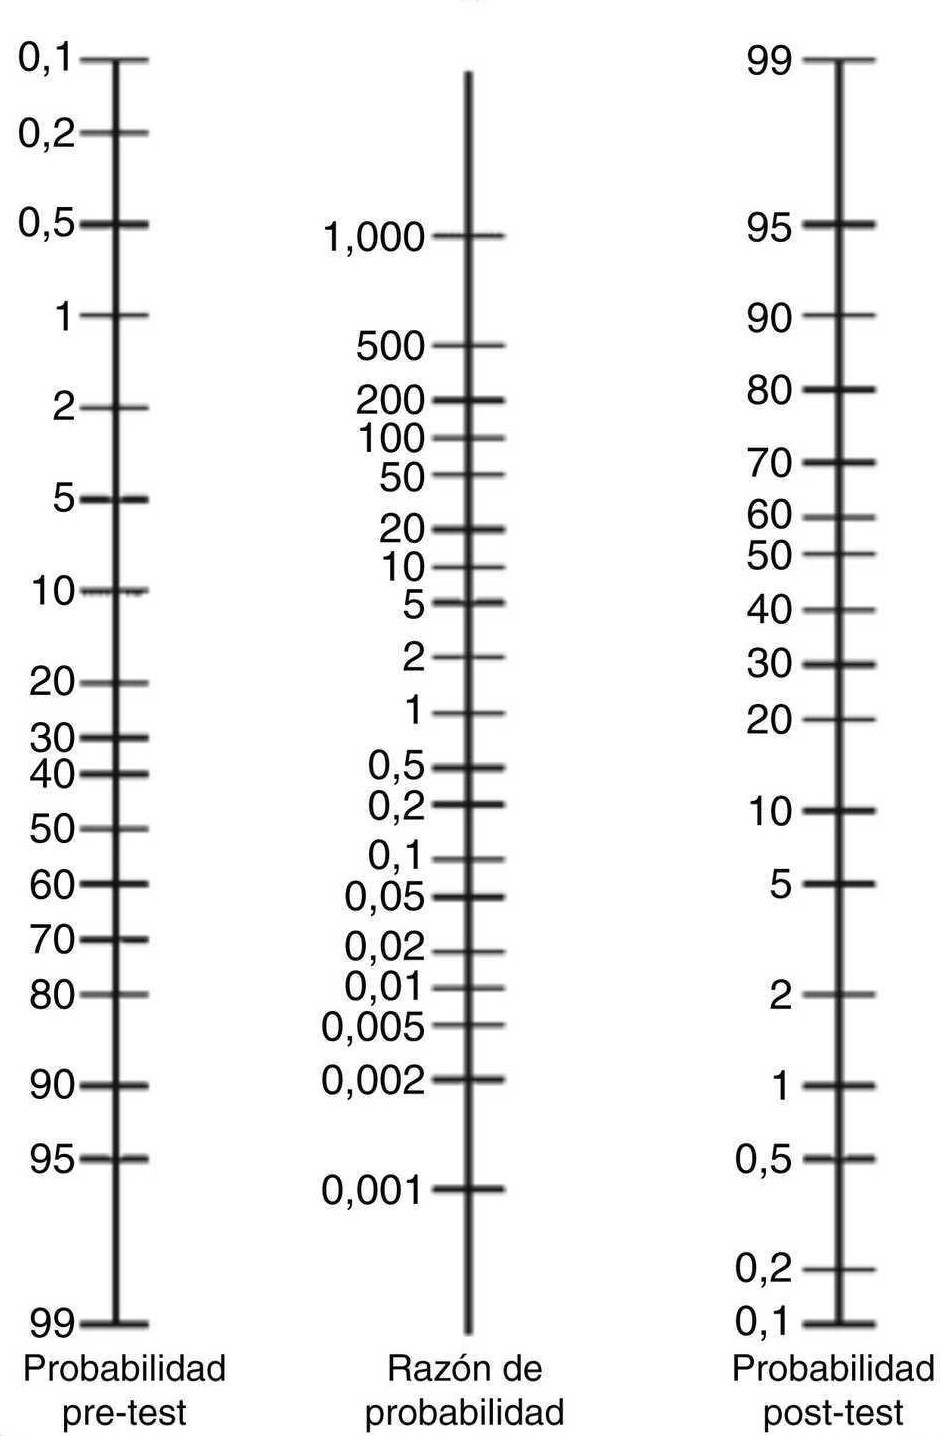
\includegraphics[scale=0.28]{Figures/nomograma.jpeg}
\caption{Nomograma de Fagan, donde línea izquierda son las probabilidades previas a la prueba, la linea central es el LR y línea derecha son las probabilidades de tener la enfermedad después del uso de la prueba.}
\label{nomograma}
\end{figure}

\section{Caso práctico}

Para la aplicación del teorema de Bayes, en este trabajo se realizó un análisis para estimar de que tan probable es que un paciente con prueba positiva por Covid\textendash 19 pueda tener la enfermedad o si el resultado es negativo, que tan probable fue que no padeciera de ella, para lo cual se utilizan los valores predictivos positivos (VPP) o negativos (VPN). Para el cálculo de estos valores, se hace necesario conocer datos como la prevalencia estimada de la enfermedad, la sensibilidad y especificidad de la prueba. Dado que las pruebas por Covid\textendash 19 en México se han confirmaron mediante RT-PCR en tiempo real y, aproximadamente, a partir del mes de septiembre el IMMS empezó a utilizar pruebas rápidas en sus hospitales con el objetivo es diferenciar rápidamente el Covid\textendash 19 de la influenza, se investigó tanto la sensibilidad como especificidad que tienen ambas pruebas.

De acuerdo a Díaz-Jiménez \cite{sensibilidad}, las pruebas PCR tienen una especificidad cercana al $100\%$ y una sensibilidad entre el $60\%$ y $80\%$ y, para las pruebas rápidas la sensibilidad más baja es del $20\%$. Sin embargo, de acuerdo a las especificaciones de las pruebas PCR, se indica que la sensibilidad alcanza un $99\%$. Para hallar la prevalencia, según la investigación de Lewis \cite{link2}, se calcula de acuerdo a la magnitud de brote y la determina mediante la ecuación \ref{prevalencia}. Por otro lado, en la investigación de Good \cite{link4}, la prevalencia podría ser también una probabilidad previa a la prueba, es decir, una probabilidad de la enfermedad con base en la sospecha clínica,
\begin{equation}
\text{prevalencia}= \frac{\text{Total casos por Covid\textendash 19}}{\text{Población total}}.
\label{prevalencia}
\end{equation}

Para efectos del presente trabajo, se consideraron dos escenarios con respecto al valor de la prevalencia. En el escenario 1, la prevalencia se calculó mediante la ecuación \ref{prevalencia}, por lo tanto, de acuerdo a la base de datos proporcionada por Hasell \cite{basededatos} a octubre 25 de 2020, hay $891,160$ total de casos por Covid\textendash 19 y la población de México es de, aproximadamente, $128,932,753$ habitantes, entonces, la prevalencia para el escenario 1 es igual a $0,691\%$ ($0.00691$).

Para el escenario 2, se contemplan dos prevalencias o probabilidades previas a la prueba por infección con Covid\textendash 19. Una probabilidad de prevalencia baja del $2\%$ y una alta del $80\%$.

Para ambos escenarios se asumió una sensibilidad para las pruebas rápidas del $20\%$ y para las pruebas PCR la sensibilidad del $80\%$ y $99\%$, La especificidad tanto para los escenarios, como para los tipos de pruebas varían entre el $99\%$ y $99,9\%$. El cálculo los valores predictivos positivos y negativos se realizaron mediante las ecuaciones \ref{vpp} y \ref{vpn}, respectivamente, basado en la investigación de \cite{bayes},
\begin{equation}
\text{VPP}= \frac{\text{sensibilidad} * \text{prevalencia}}{\text{sensibilidad} * \text{prevalencia} + (1- \text{sensibilidad})*(1-\text{especificidad})},
\label{vpp}
\end{equation}
\begin{equation}
\text{VPN}= \frac{\text{especificidad} * (1- \text{prevalencia})}{(1- \text{sensibilidad}) * \text{prevalencia} + \text{especificidad} * (1- \text{prevalencia})}.
\label{vpn}
\end{equation}

Es importante tener en cuenta que los VPP estiman la probabilidad condicional de que la persona pueda estar enferma cuando la prueba ha dado positiva y los VPN es la ``capacidad de descartar una enfermedad" dado un resultado negativo en la prueba, por lo tanto, para determinar la probabilidad condicional de que una persona pueda estar enferma dado que su prueba es negativa (falso negativo) será igual a $1 -$VPN. 

\begin{table}
\centering
\caption{Estimación de la probabilidad condicional para las pruebas por Covid\textendash 19}
\begin{tabular}{|c|c|c|c|r|r|}
\hline
\multirow{2}{*}{\textbf{Escenario}} & \multirow{3}{*}{\textbf{\begin{tabular}[c]{@{}c@{}}Prevalencia\\ ($\%$)\end{tabular}}} & \multirow{3}{*}{\textbf{\begin{tabular}[c]{@{}c@{}}Especificidad\\ ($\%$)\end{tabular}}} & \multirow{3}{*}{\textbf{\begin{tabular}[c]{@{}c@{}}Sensibilidad\\ ($\%$)\end{tabular}}} & \multicolumn{2}{c|}{\textbf{Teorema de Bayes}}                                                                                                        \\ \cline{5-6} 
                                    &                                                                                        &                                                                                          &                                                                                         & \textbf{\begin{tabular}[c]{@{}c@{}}Prueba positiva\\ ($\%$)\end{tabular}} & \textbf{\begin{tabular}[c]{@{}c@{}}Prueba negativa\\ ($\%$)\end{tabular}} \\ \hline
\multirow{6}{*}{1}                  & \multirow{6}{*}{0.691}                                                                 & \multirow{3}{*}{99.0}                                                                    & 20                                                                                      & 12.2                                                                      & 0.6                                                                       \\ \cline{4-6} 
                                    &                                                                                        &                                                                                          & 80                                                                                      & 35.8                                                                      & 0.1                                                                       \\ \cline{4-6} 
                                    &                                                                                        &                                                                                          & 99                                                                                      & 40.8                                                                      & 0.0                                                                       \\ \cline{3-6} 
                                    &                                                                                        & \multirow{3}{*}{99.9}                                                                    & 20                                                                                      & 58.2                                                                      & 0.6                                                                       \\ \cline{4-6} 
                                    &                                                                                        &                                                                                          & 80                                                                                      & 84.8                                                                      & 0.1                                                                       \\ \cline{4-6} 
                                    &                                                                                        &                                                                                          & 99                                                                                      & 87.3                                                                      & 0.0                                                                       \\ \hline
\multirow{12}{*}{2}                 & \multirow{6}{*}{2}                                                                     & \multirow{3}{*}{99.0}                                                                    & 20                                                                                      & 29.0                                                                       & 1.6                                                                       \\ \cline{4-6} 
                                    &                                                                                        &                                                                                          & 80                                                                                      & 62.0                                                                      & 0.4                                                                       \\ \cline{4-6} 
                                    &                                                                                        &                                                                                          & 99                                                                                      & 66.9                                                                      & 0.0                                                                       \\ \cline{3-6} 
                                    &                                                                                        & \multirow{3}{*}{99.9}                                                                    & 20                                                                                      & 80.3                                                                      & 1.6                                                                       \\ \cline{4-6} 
                                    &                                                                                        &                                                                                          & 80                                                                                      & 94.2                                                                      & 0.4                                                                       \\ \cline{4-6} 
                                    &                                                                                        &                                                                                          & 99                                                                                      & 95.3                                                                      & 0.0                                                                       \\ \cline{2-6} 
                                    & \multirow{6}{*}{80}                                                                    & \multirow{3}{*}{99.0}                                                                    & 20                                                                                      & 98.8                                                                      & 76.4                                                                      \\ \cline{4-6} 
                                    &                                                                                        &                                                                                          & 80                                                                                      & 99.7                                                                      & 44.7                                                                      \\ \cline{4-6} 
                                    &                                                                                        &                                                                                          & 99                                                                                      & 99.7                                                                      & 3.9                                                                       \\ \cline{3-6} 
                                    &                                                                                        & \multirow{3}{*}{99.9}                                                                    & 20                                                                                      & 99.9                                                                      & 76.2                                                                      \\ \cline{4-6} 
                                    &                                                                                        &                                                                                          & 80                                                                                      & 100.0                                                                     & 44.5                                                                      \\ \cline{4-6} 
                                    &                                                                                        &                                                                                          & 99                                                                                      & 100.0                                                                      & 3.8                                                                       \\ \hline
\end{tabular}
\label{resultados}
\end{table}

Considerando lo antes mencionado y los resultados del cuadro \ref{resultados}, observamos que al comparar la efectividad o sensibilidad del $99\%$ en un resultado positivo a través de las pruebas de PCR, con la probabilidad condicional, si se considera la prevalencia con respecto a la magnitud del brote (prevalencia muy baja ($0.691\%$), da como resultado una estimación de la efectividad de la prueba del $41\%$ y $87\%$, con especificidades del $99\%$ y $99.9\%$, respectivamente. Mientras que, si se considera una prevalencia alta, es decir, con base al riesgo al que ha estado expuesta la persona, la probabilidad condicional estimada para la efectividad de la prueba oscila entre el $96\%$ y $100\%$. Por lo anterior, se podría llegar a un resultado contraintuitivo, ya que la probabilidad de que una persona con un resultado positivo a través de las pruebas PCR se pueda determinar como un posible caso verdadero con Covid\textendash 19, oscila entre un $41\%$ y $87\%$ y no con una probabilidad del $99\%$ como se ha especificado para este tipo de pruebas, aunque este resultado depende de la prevalencia considerada, como se observa en la figura \ref{resultadovpp}.

De igual manera, cuando los resultados de las pruebas son negativos, se observa que mientras la prevalencia aumenta, también aumenta la probabilidad de falsos negativos, siendo, principalmente, un foco de atención las pruebas con sensibilidad muy baja, ya que se muestra una probabilidad muy alta (aproximadamente del $76\%$) de que las personas con resultados negativos por Covid\textendash 19, no estén posiblemente sin la enfermedad, es decir, un aumento de la tasa en los falsos negativos. Por lo tanto, un resultado negativo obtenido por las pruebas rápidas (sensibilidad del $20\%$), no sería un buen indicador para descartar la existencia de la enfermedad, ya que como podemos observar en el cuadro \ref{resultados}, con una prevalencia baja o alta, se presenta la probabilidad más alta de falsos negativos. No obstante, considerando que el resultado sea positivo, es posible que puedan ser de utilidad ya que la probabilidad condicional estimada es relativamente buena comparada las pruebas PCR a medida que aumenta la prevalencia, como se observa en la figura \ref{resultadovpp}.

\begin{figure}[h]
\centering
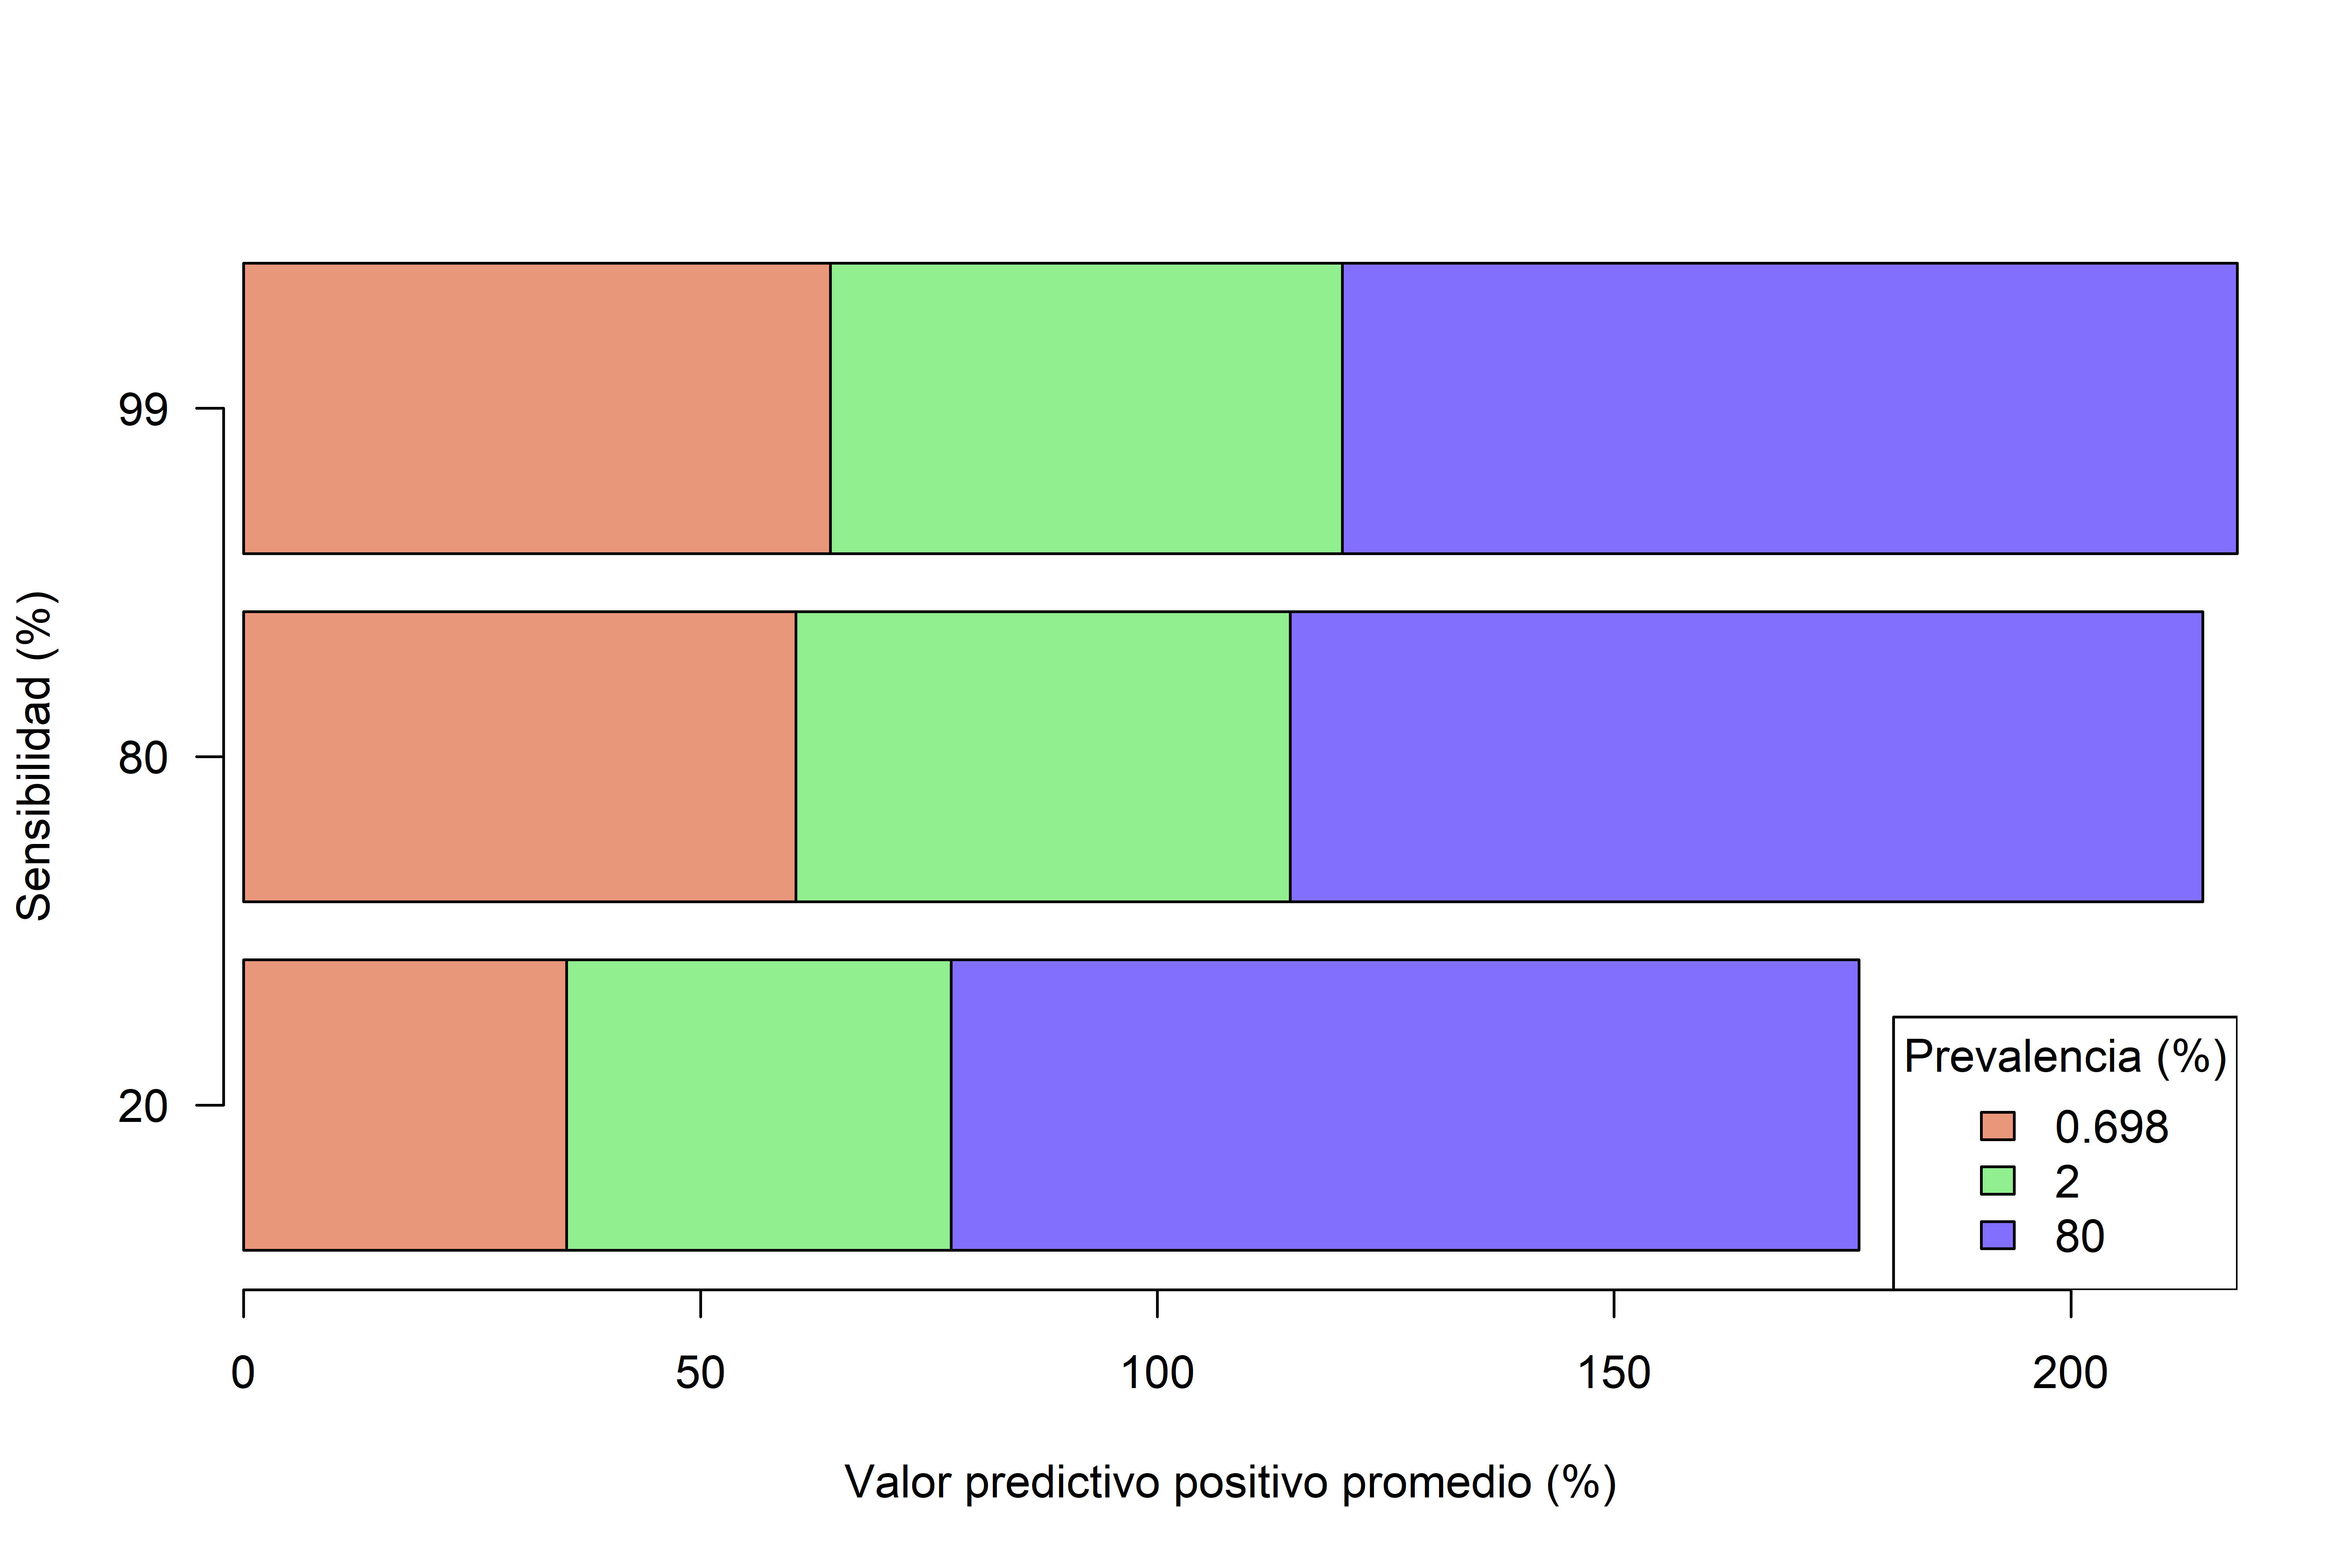
\includegraphics[scale=0.6]{Figures/vpp.png}
\caption{Valores predictivos positivos promedio}
\label{resultadovpp}
\end{figure}

Como conclusión general, para las pruebas PCR, mediante el teorema de Bayes, es decir, por medio de los VPP y VPN si se considera un muestreo masivo de la población, determinar si la eficiencia de la prueba es alta, depende de la prevalencia real de la enfermedad del lugar donde se aplica, en este caso, de la magnitud del brote. Sin embargo, cuando el muestreo se considera con base a sectores donde se ha comprobado una mayor prevalencia o riesgo de contagio, la eficiencia (sensibilidad) reportada de la prueba ayuda a estimar con una mayor probabilidad la detección de casos en la población y, de esta manera aplicar las medidas de control necesarias. La base de datos y el código en R utilizado, se encuentran disponibles en el repositorio de GitHub \cite{github}.

\bibliography{refProbabilidad}
\bibliographystyle{plain}

\end{document}

